\documentclass[12pt,a4paper]{article}
\usepackage[utf8]{inputenc}
\usepackage[spanish]{babel}
\usepackage{mathptmx}
\usepackage{graphicx}
\usepackage{geometry}
\geometry{top=2.54cm, bottom=2.54cm, left=2.54cm, right=2.54cm}
\usepackage{float}
\usepackage{hyperref}
\usepackage{url}
\usepackage{booktabs}
\usepackage{amsmath}

\usepackage{setspace}
\doublespacing
\usepackage{indentfirst}
\setlength{\parindent}{1.27cm}

\usepackage{caption}
\captionsetup[figure]{name=Figura, labelsep=newline, justification=raggedright, singlelinecheck=false, labelfont=bf, textfont=it}
\captionsetup[table]{labelsep=newline, justification=raggedright, singlelinecheck=false, labelfont=bf, textfont=it}

\usepackage{titlesec}
\titleformat{\section}[block]{\normalfont\normalsize\bfseries\centering}{}{0em}{}
\titleformat{\subsection}[block]{\normalfont\normalsize\bfseries}{}{0em}{}

\begin{document}

% ---------------------------------------------------------
% PORTADA
% ---------------------------------------------------------
\begin{titlepage}
    \singlespacing
    \setlength{\parindent}{0cm}
    \centering
    {\bfseries\Large UNIVERSIDAD NACIONAL DEL ALTIPLANO \par}
    \vspace{0.4cm}
    {\bfseries\large FACULTAD DE INGENIERÍA DE MECÁNICA ELÉCTRICA, INGENIERÍA ELECTRÓNICA E INGENIERÍA DE SISTEMAS \par}
    \vspace{0.4cm}
    {\bfseries\large ESCUELA PROFESIONAL DE INGENIERÍA DE SISTEMAS \par}
    
    \vspace{0.8cm}
    
\includegraphics[width=0.35\textwidth]{imagenes/logo.png}\par
    \vspace{0.8cm}
    
    {\bfseries\Large Interfaz de la gestión de disco (Nuevas Asignaciones) \par}
    
    \vspace{1.2cm}
    
    {\bfseries CURSO.} \par
    SISTEMAS OPERATIVOS \par
    
    \vspace{0.5cm}
    {\bfseries DOCENTE.} \par
    RUELAS ACERO DONIA ALIZANDRA \par
    
    \vspace{0.5cm}
    {\bfseries ALUMNO.} \par
    ABAD POMA MAQUERA \par
    
    \vspace{0.5cm}
    {\bfseries CODIGO.} \par
    241177 \par
    
    \vspace{0.5cm}
    {\bfseries QUINTO SEMESTRE} \par
    {\bfseries 2026 – I} \par
    
    \vfill
    {\bfseries PUNO – PERÚ} \par
\end{titlepage}

\newpage
\doublespacing
\setlength{\parindent}{1.27cm}

\section{Introducción}
La gestión eficiente del almacenamiento requiere esquemas robustos, dado que las estrategias básicas (contigua y enlazada) presentan limitaciones significativas en entornos de producción. Para analizar visualmente la teoría, se ampliaron las capacidades del simulador interactivo \textit{SimuKernel}, incorporando cuatro métodos avanzados: Tabla de Asignación de Archivos (FAT), Indexación Multi-Nivel, asignación por Extensiones (Extents) y gestión de espacio libre mediante Mapa de Bits (Bitmap). El propósito es evidenciar cómo estas lógicas mitigan problemas clásicos, como la fragmentación y el alto costo de lectura, optimizando el rendimiento del disco.

\section{Objetivo General}
Documentar el funcionamiento de las técnicas avanzadas de asignación en disco (FAT, Indexada Multi-Nivel, Extensiones y Bitmap) a través del simulador interactivo, evaluando su impacto en el rendimiento general, la fragmentación externa y las operaciones de entrada/salida (E/S).

\section{Marco Teórico}
El método FAT mejora la asignación enlazada al extraer y centralizar los punteros en una tabla ubicada al inicio del disco. Si un archivo ocupa los bloques 2, 8 y 14, el directorio solo referencia al bloque 2. La tabla FAT vincula secuencialmente estas posiciones hasta marcar el fin del archivo. Esto permite aprovechar la capacidad total de los bloques físicos para almacenar datos y agiliza las búsquedas, ya que la tabla completa se carga en la memoria RAM.

\subsection{Indexada Multi-Nivel}
La indexación simple utiliza un bloque exclusivo para listar los punteros de un archivo, pero resulta insuficiente para archivos de gran tamaño. La indexación multi-nivel resuelve esta limitación estructurando los punteros jerárquicamente. Un índice primario (nivel 1) apunta a índices secundarios (nivel 2), los cuales finalmente referencian los bloques de datos. Esta arquitectura expande exponencialmente la capacidad de almacenamiento, siendo la base de sistemas de archivos como ext3.

\subsection{Asignación por Extensiones (Extents)}
Una extensión es una agrupación de bloques físicos contiguos. En lugar de registrar cada bloque individual, el sistema almacena únicamente la dirección de inicio y la longitud del conjunto. Si un archivo requiere 50 bloques, se registra como una sola extensión de longitud 50. Si el archivo crece y carece de espacio adyacente, se crea una nueva extensión. Este modelo equilibra la velocidad de lectura secuencial con la flexibilidad para escalar.

\subsection{Mapa de Bits (Bitmap)}
El mapa de bits gestiona el espacio libre representando cada bloque del disco con un bit: '0' indica disponibilidad y '1' ocupación. Una secuencia inicial de cuatro bloques ocupados y tres libres se representa como \texttt{1111000}. Esta técnica optimiza la asignación, ya que los procesadores modernos ejecutan operaciones binarias a alta velocidad para identificar cadenas de ceros contiguos, reemplazando la lenta iteración sobre listas textuales.

\section{Arquitectura de Simulación y Modalidades}

El núcleo del simulador fue actualizado para albergar siete métodos de asignación (Contigua, Enlazada, Indexada, FAT, Indexada Multi-Nivel, Extensiones y Bitmap), permitiendo comparar objetivamente el rendimiento entre arquitecturas clásicas y modernas.

\begin{figure}[H]
    \caption{\textit{Panel principal de parámetros exhibiendo los siete algoritmos disponibles y las modalidades de asignación.}}
    \centering
    \vspace{0.3cm}
    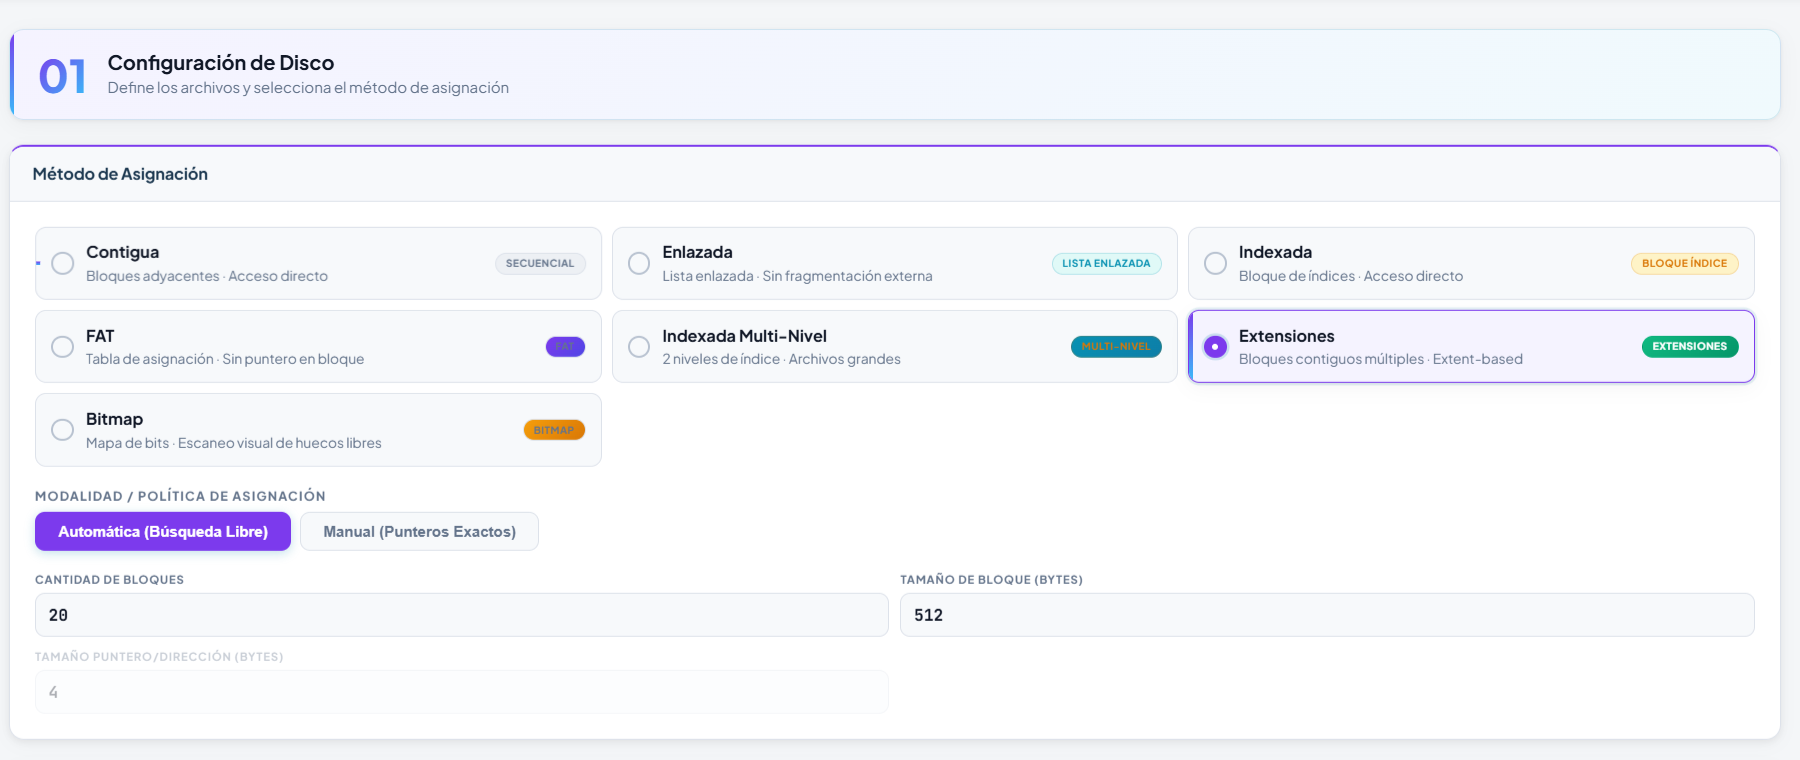
\includegraphics[width=0.9\textwidth]{imagenes/param_general.png}
\end{figure}

El sistema distingue dos modalidades operativas para la asignación de espacio:
\begin{itemize}
    \item \textbf{Modalidad Manual (Punteros Exactos):} Permite definir explícitamente la ubicación física de los bloques, índices o extensiones. Resulta esencial para comprender la lógica matemática detrás de las referencias internas.
    \item \textbf{Modalidad Automática (Búsqueda Libre):} Delega la asignación al núcleo simulado. A partir del tamaño requerido, el sistema escanea el almacenamiento utilizando estructuras como el mapa de bits para localizar espacio disponible y construir las tablas de asignación de manera autónoma.
\end{itemize}

\section{Descripción de los Algoritmos y su Lógica}
En la \textbf{asignación FAT}, el simulador mantiene en memoria un arreglo paralelo al disco. Durante la asignación, los bloques físicos almacenan visualmente los datos, mientras que los punteros se estructuran de forma independiente en un panel lateral de metadatos.

Para la \textbf{Indexada Multi-Nivel}, el modelo valida estrictamente la jerarquía. El motor visual traza las operaciones simulando el retraso (\textit{overhead}) originado al acceder primero al bloque raíz, luego a los subíndices y, finalmente, a los datos.

La lógica de \textbf{Extensiones} procesa iterativamente pares de datos (inicio, longitud). El algoritmo previene la superposición de bloques y representa gráficamente grandes franjas unificadas, consolidando cada extensión lógica en una única referencia de directorio.

El \textbf{Mapa de Bits} opera como un observador en segundo plano. Antes de asignar bloques, el simulador genera un arreglo binario. Durante la ejecución, el algoritmo escanea este arreglo para localizar espacios disponibles, actualizando en tiempo real un panel visual que refleja la transición lógica de ceros a unos.

\section{Métricas y su Influencia}
La elección del método incide directamente en los indicadores del sistema:

\begin{itemize}
    \item \textbf{Fragmentación Externa:} Mide los espacios libres dispersos. Las Extensiones mitigan este problema agrupando datos en áreas contiguas. En contraste, FAT y la asignación Indexada la eliminan por completo, ya que pueden direccionar cualquier bloque aislado.
    \item \textbf{Operaciones E/S:} Cuantifica las lecturas y escrituras físicas. La Indexada Multi-Nivel registra valores elevados debido a las lecturas previas de sus índices jerárquicos. FAT y Extensiones optimizan estas operaciones, manteniendo métricas significativamente más bajas.
    \item \textbf{Uso del Disco (\%):} Refleja la densidad de almacenamiento. La Indexada Multi-Nivel requiere bloques exclusivos para estructurar índices, lo que eleva el porcentaje de ocupación global incluso con archivos de menor tamaño.
\end{itemize}

\section{Resultados de la Simulación}

A continuación, se presentan los escenarios de prueba para los cuatro métodos avanzados, incluyendo su respectiva configuración de entrada (parámetros) y el resultado gráfico final producido por el simulador.

\subsection{Simulación FAT}

Para evaluar FAT, se ingresaron secuencias de bloques dispersos. Se evidenció la ausencia de fragmentación externa y el aprovechamiento total del espacio en los bloques de datos, prescindiendo del almacenamiento interno de punteros.

\begin{table}[H]
    \centering
    \caption{\textit{Datos de entrada para simulación FAT}}
    \vspace{0.3cm}
    \begin{tabular}{ll}
        \toprule
        \textbf{Archivo} & \textbf{Punteros Lógicos (Secuencia)} \\
        \midrule
        FILE1 & 2, 8, 14, 25 \\
        FILE2 & 5, 6, 7 \\
        \bottomrule
    \end{tabular}
\end{table}

\begin{figure}[H]
    \caption{\textit{Configuración de los parámetros y carga de datos para el método FAT.}}
    \centering
    \vspace{0.3cm}
    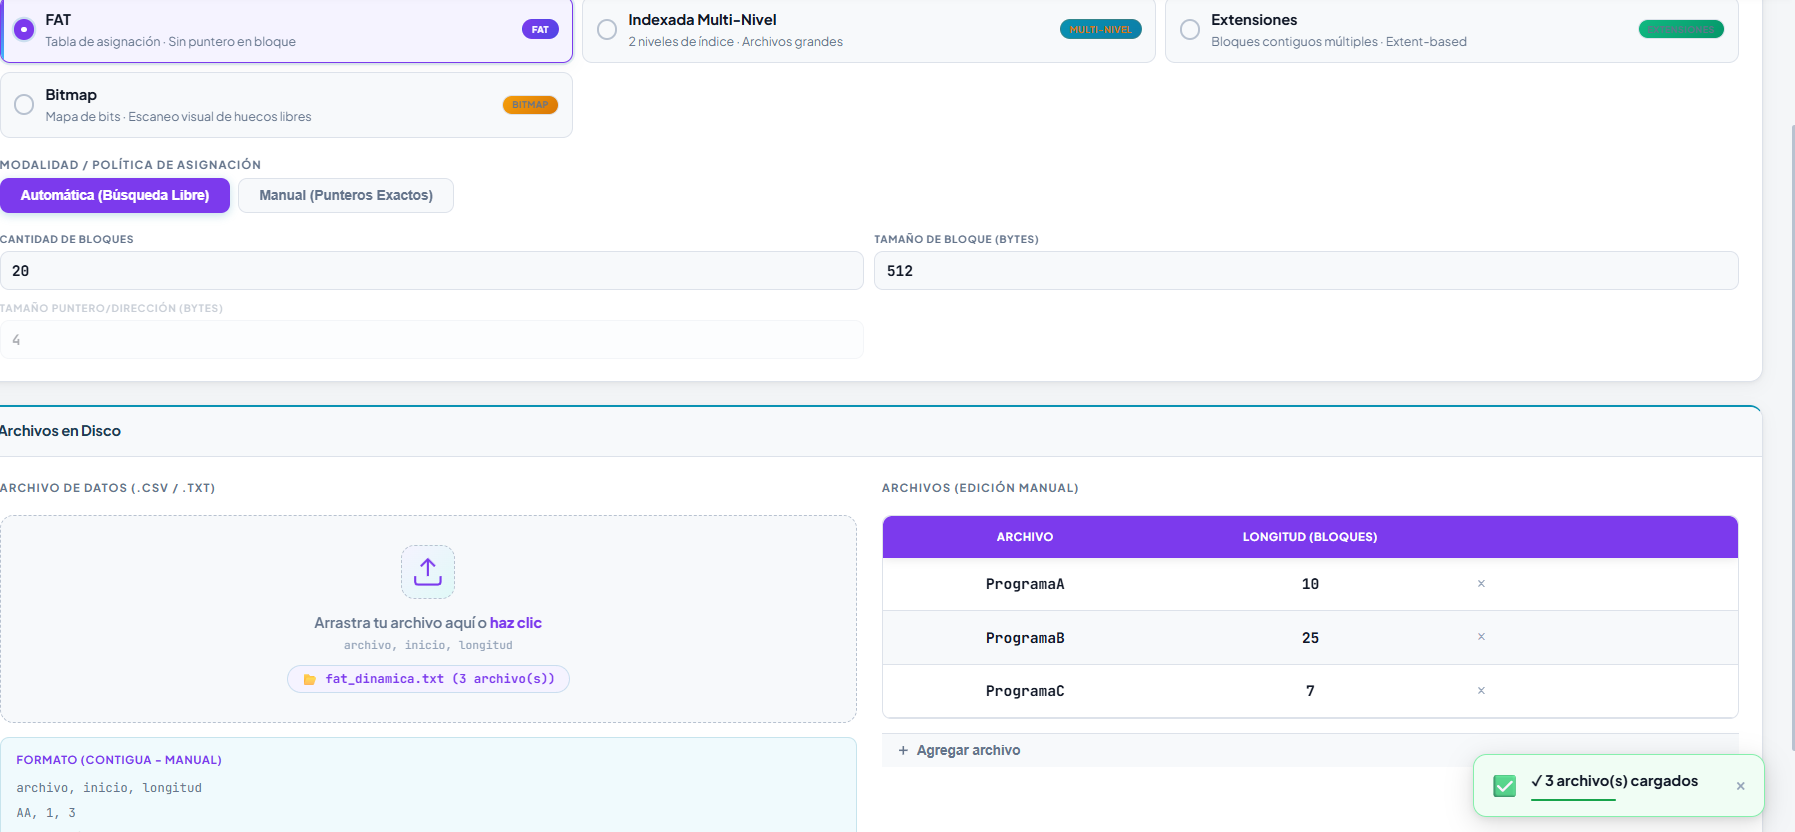
\includegraphics[width=0.9\textwidth]{imagenes/param_fat.png}
\end{figure}

\begin{figure}[H]
    \caption{\textit{Estado final del disco usando FAT. Nótese la limpieza en los bloques de datos.}}
    \centering
    \vspace{0.3cm}
    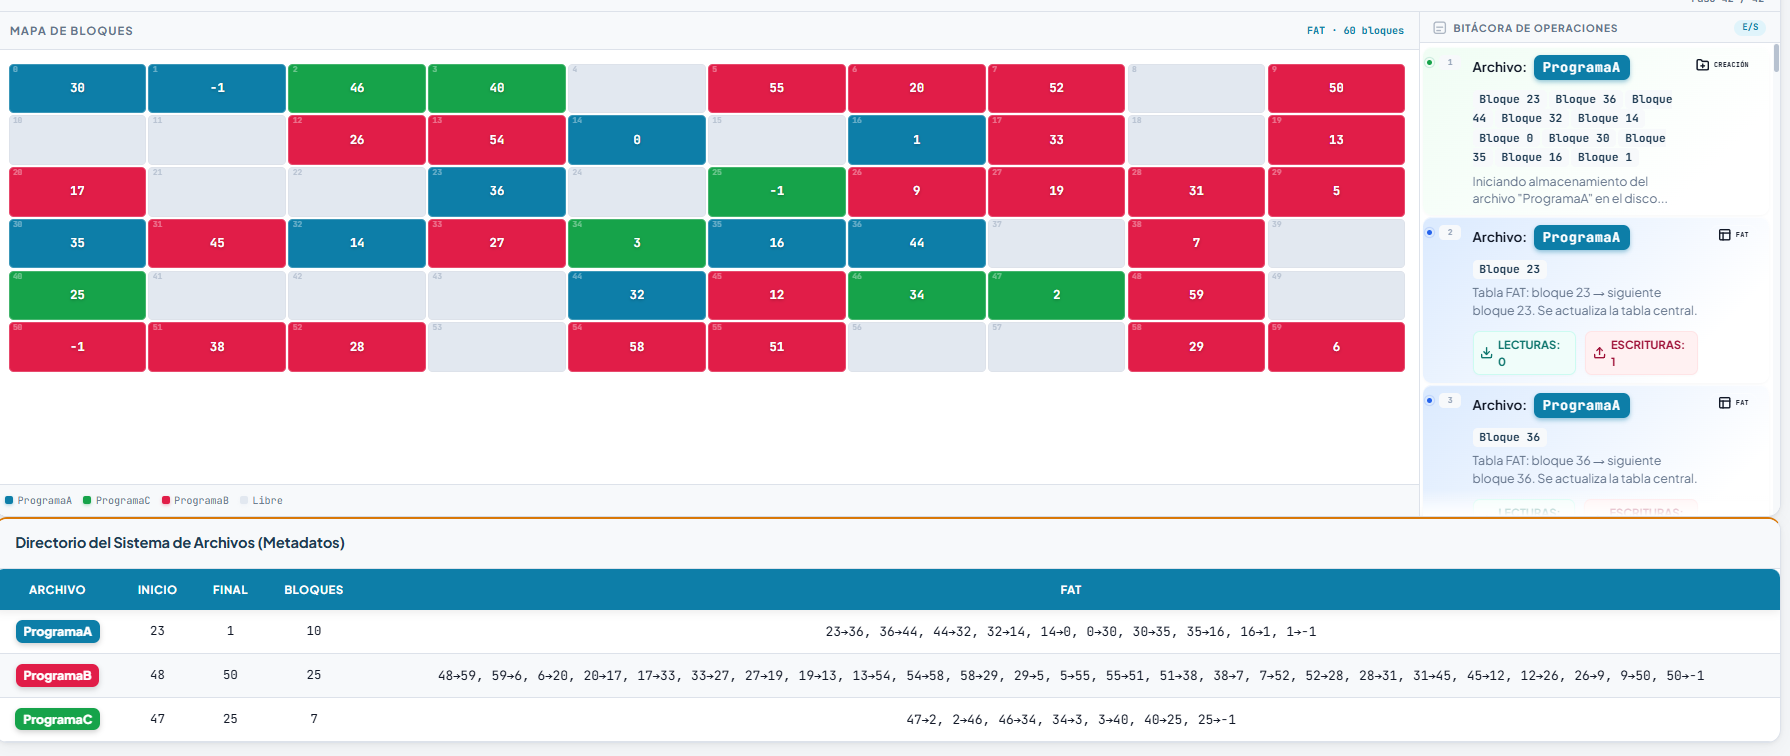
\includegraphics[width=1\textwidth]{imagenes/sim_fat.png}
\end{figure}

Durante la ejecución, la ocupación física emuló el comportamiento de una lista enlazada, pero centralizando íntegramente la gestión de referencias en el directorio externo. 

\subsection{Simulación Indexada Multi-Nivel}

Se configuró un bloque maestro que deriva en dos subíndices, los cuales referencian posteriormente a los bloques de datos, modelando la asignación estructurada de un archivo pesado.

\begin{table}[H]
    \centering
    \caption{\textit{Datos de entrada para simulación Indexada Multi-Nivel}}
    \vspace{0.3cm}
    \begin{tabular}{lll}
        \toprule
        \textbf{Archivo} & \textbf{Nivel 1 (Índice Raíz)} & \textbf{Nivel 2 y Datos} \\
        \midrule
        DB\_BIG & 10 & Ind1: 15 (Datos: 1,2), Ind2: 16 (Datos: 8,9) \\
        \bottomrule
    \end{tabular}
\end{table}

\begin{figure}[H]
    \caption{\textit{Carga de parámetros y definición explícita de los niveles de indexación.}}
    \centering
    \vspace{0.3cm}
    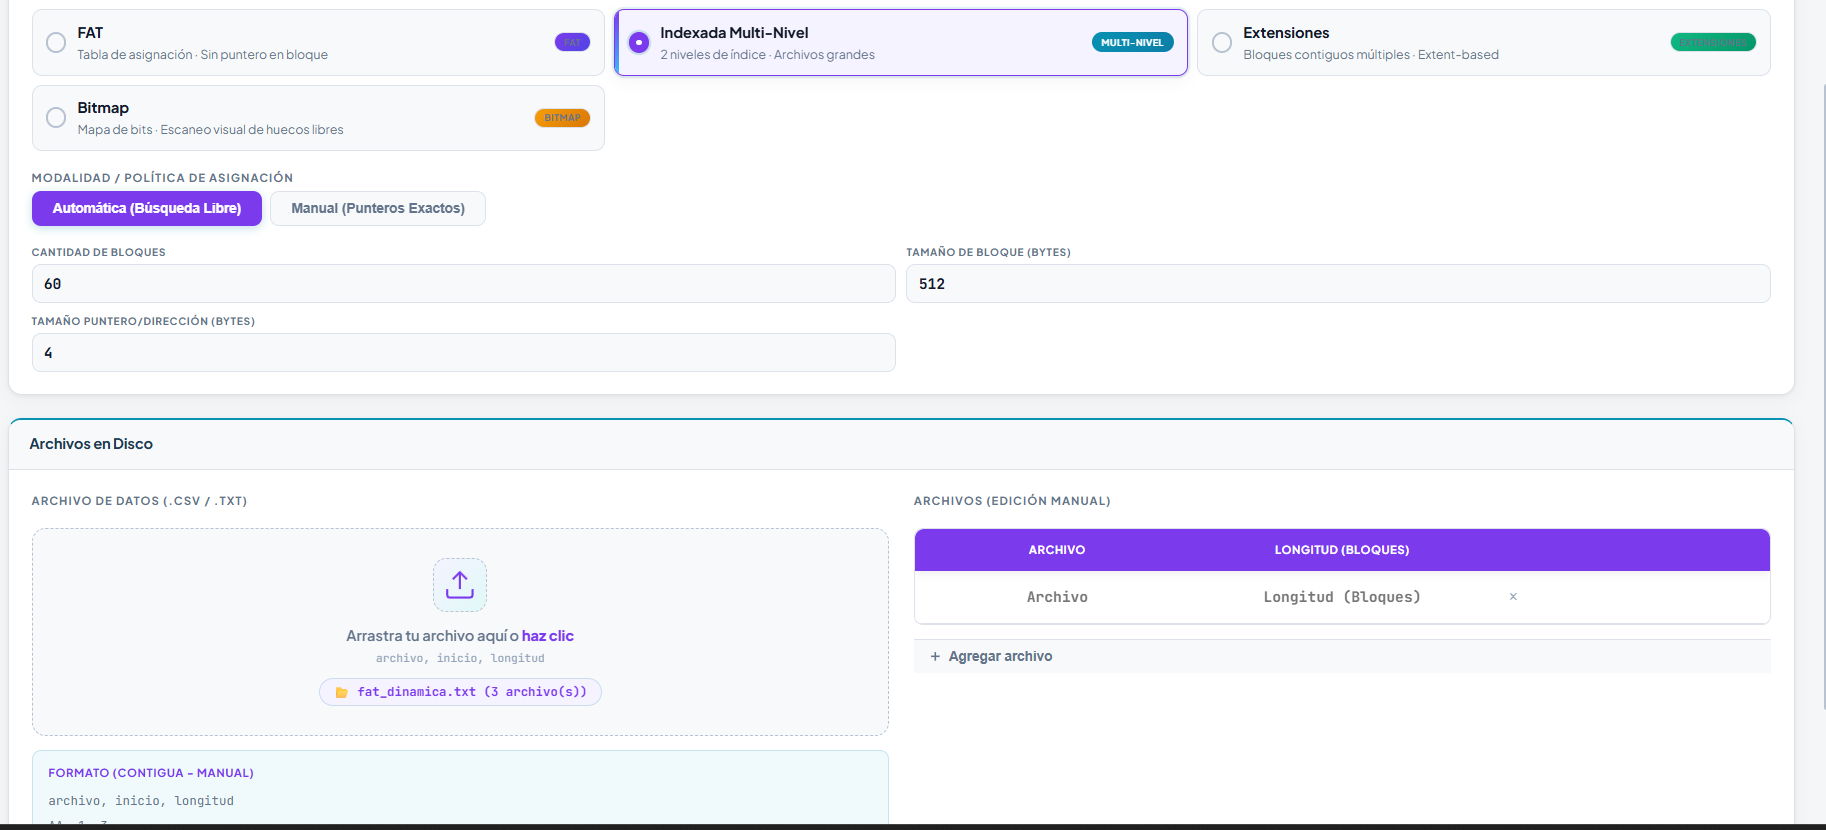
\includegraphics[width=0.9\textwidth]{imagenes/param_indexml.png}
\end{figure}

\begin{figure}[H]
    \caption{\textit{Jerarquía estructurada de bloques en Indexada Multi-Nivel.}}
    \centering
    \vspace{0.3cm}
    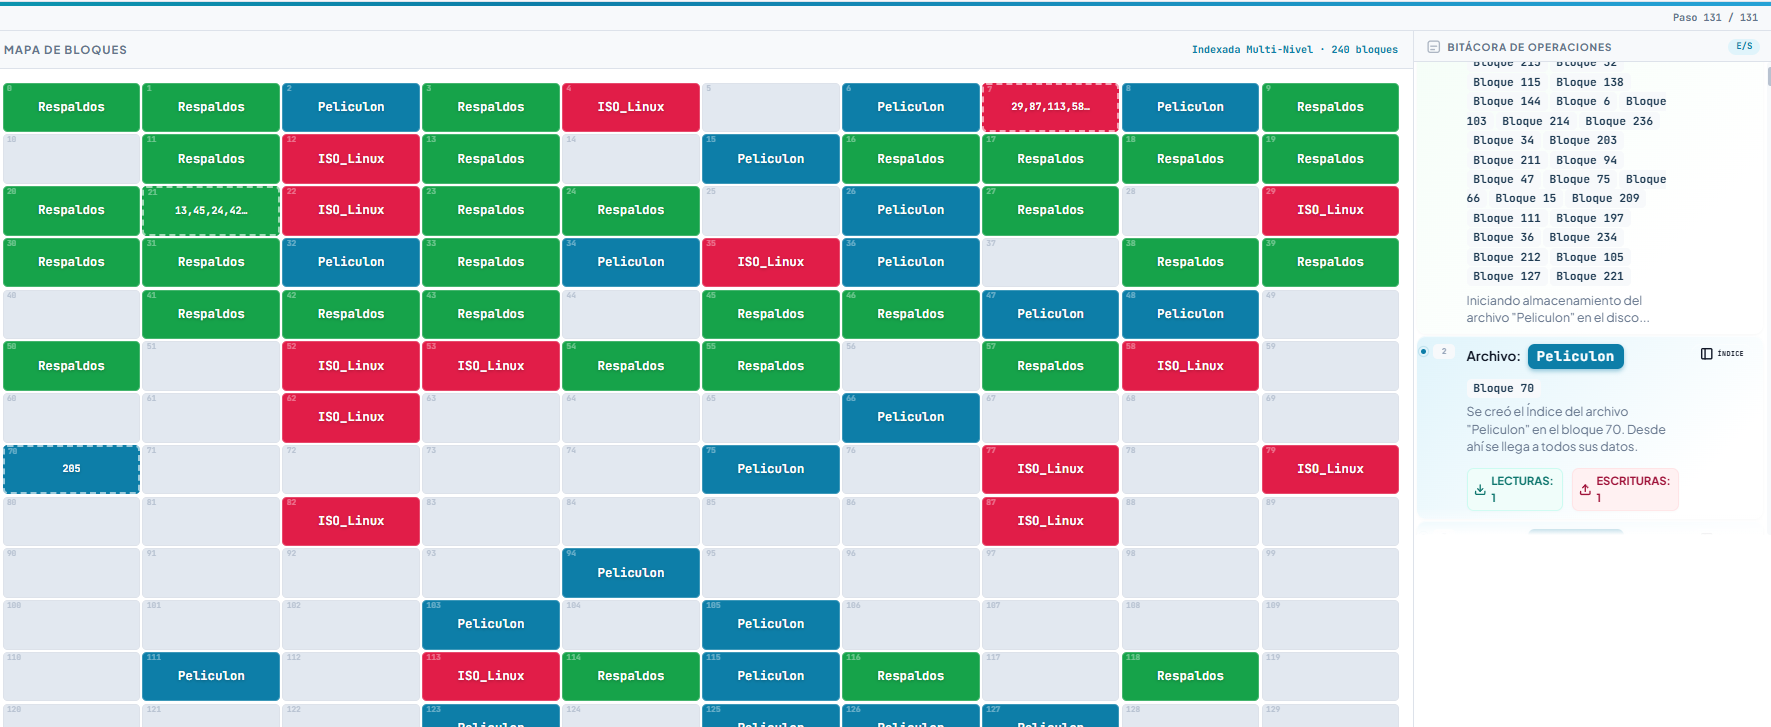
\includegraphics[width=1\textwidth]{imagenes/sim_indexml.png}
\end{figure}

La bitácora de simulación registró un volumen alto de operaciones E/S. El algoritmo requirió acceder secuencialmente al bloque raíz (10) y luego a los índices secundarios (15 y 16) antes de autorizar la lectura definitiva de los datos.

\subsection{Simulación por Extensiones}

Se simuló un escenario de fragmentación que el algoritmo resolvió agrupando la información en porciones contiguas masivas.

\begin{table}[H]
    \centering
    \caption{\textit{Datos de entrada para simulación por Extensiones}}
    \vspace{0.3cm}
    \begin{tabular}{ll}
        \toprule
        \textbf{Archivo} & \textbf{Extensiones: (Inicio, Longitud)} \\
        \midrule
        VIDEO & (5, 4); (20, 3) \\
        AUDIO & (10, 2); (40, 5) \\
        \bottomrule
    \end{tabular}
\end{table}

\begin{figure}[H]
    \caption{\textit{Definición manual de las extensiones (Extents) en el panel de entrada de datos.}}
    \centering
    \vspace{0.3cm}
    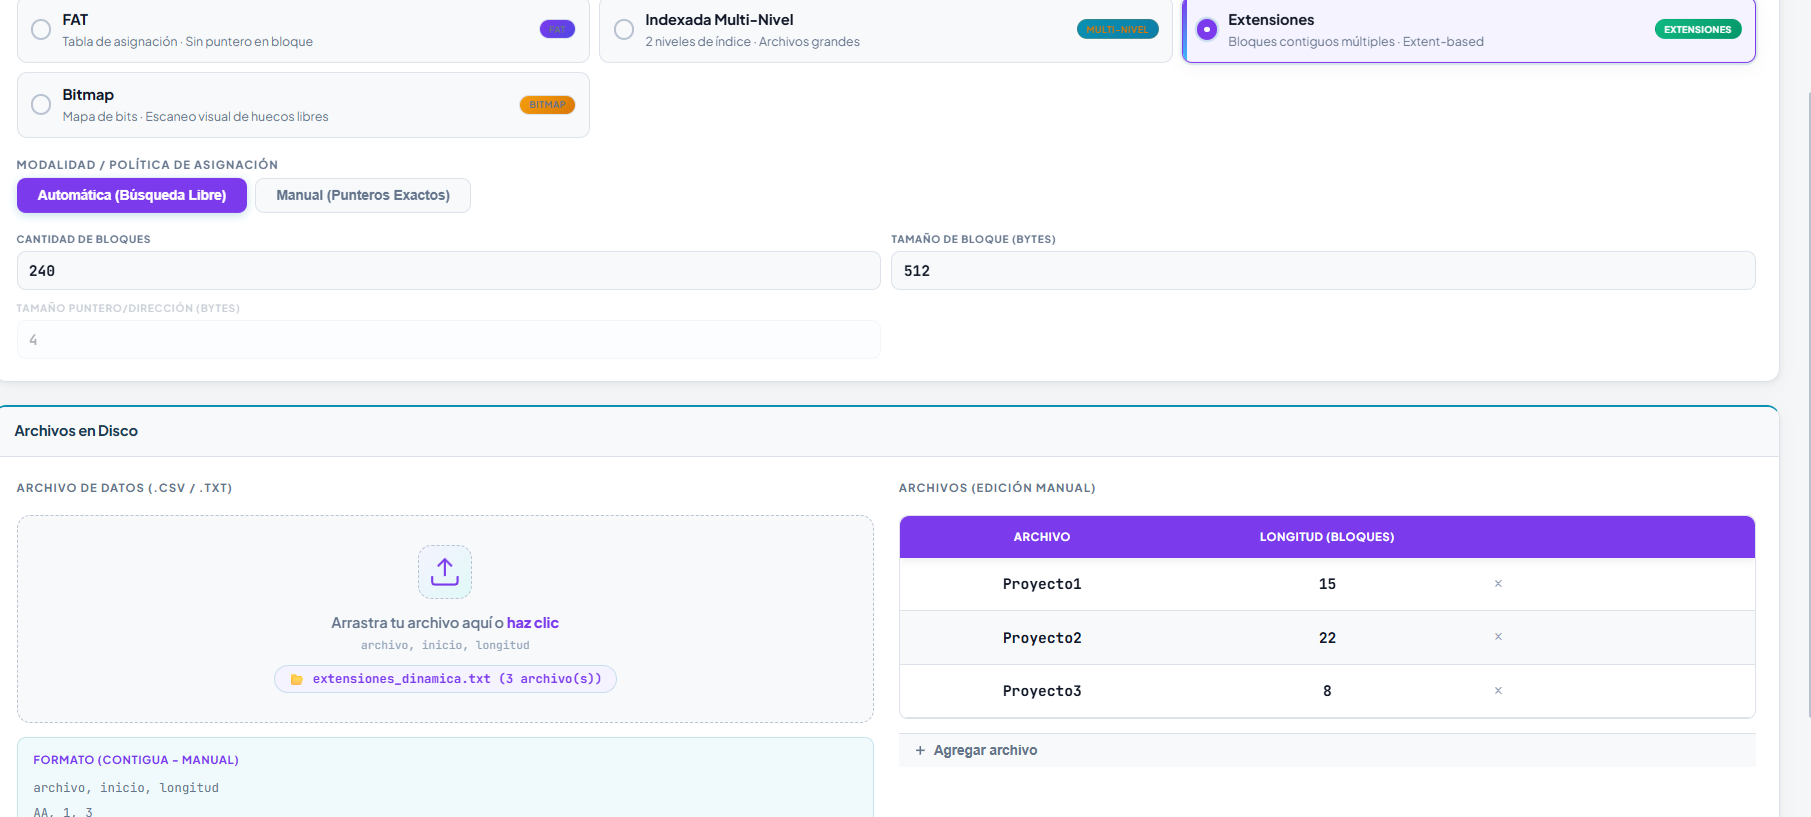
\includegraphics[width=0.9\textwidth]{imagenes/param_extensiones.png}
\end{figure}

\begin{figure}[H]
    \caption{\textit{Archivos distribuidos organizadamente por extensiones masivas en el simulador.}}
    \centering
    \vspace{0.3cm}
    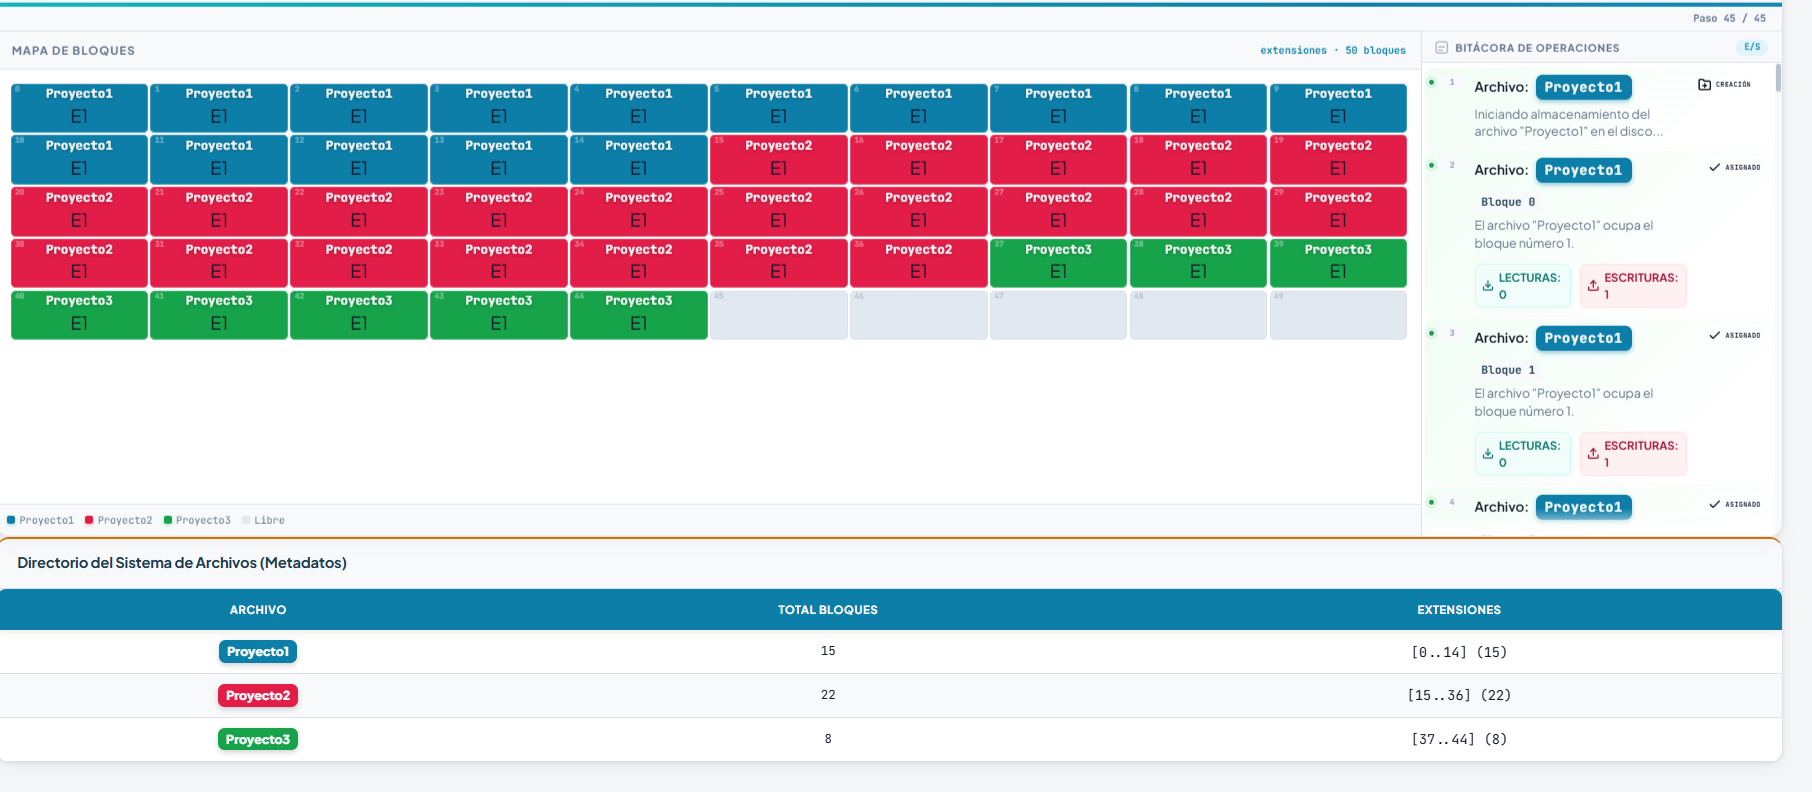
\includegraphics[width=1\textwidth]{imagenes/sim_extensiones.png}
\end{figure}

El mapeo final mostró una distribución consolidada. Los archivos se estructuraron en cadenas consistentes en lugar de bloques aislados, un patrón que incrementa drásticamente la velocidad de lectura secuencial en unidades físicas.

\subsection{Simulación Bitmap}

Se evaluó la asignación dinámica para monitorear el comportamiento del mapa de bits como estructura de control subyacente.

\begin{table}[H]
    \centering
    \caption{\textit{Datos de entrada para simulación con Bitmap}}
    \vspace{0.3cm}
    \begin{tabular}{lc}
        \toprule
        \textbf{Archivo} & \textbf{Longitud Solicitada (Bloques)} \\
        \midrule
        SYS\_LOG & 8 \\
        APP\_BIN & 15 \\
        \bottomrule
    \end{tabular}
\end{table}

\begin{figure}[H]
    \caption{\textit{Configuración en modalidad automática para Bitmap, solicitando únicamente longitudes totales.}}
    \centering
    \vspace{0.3cm}
    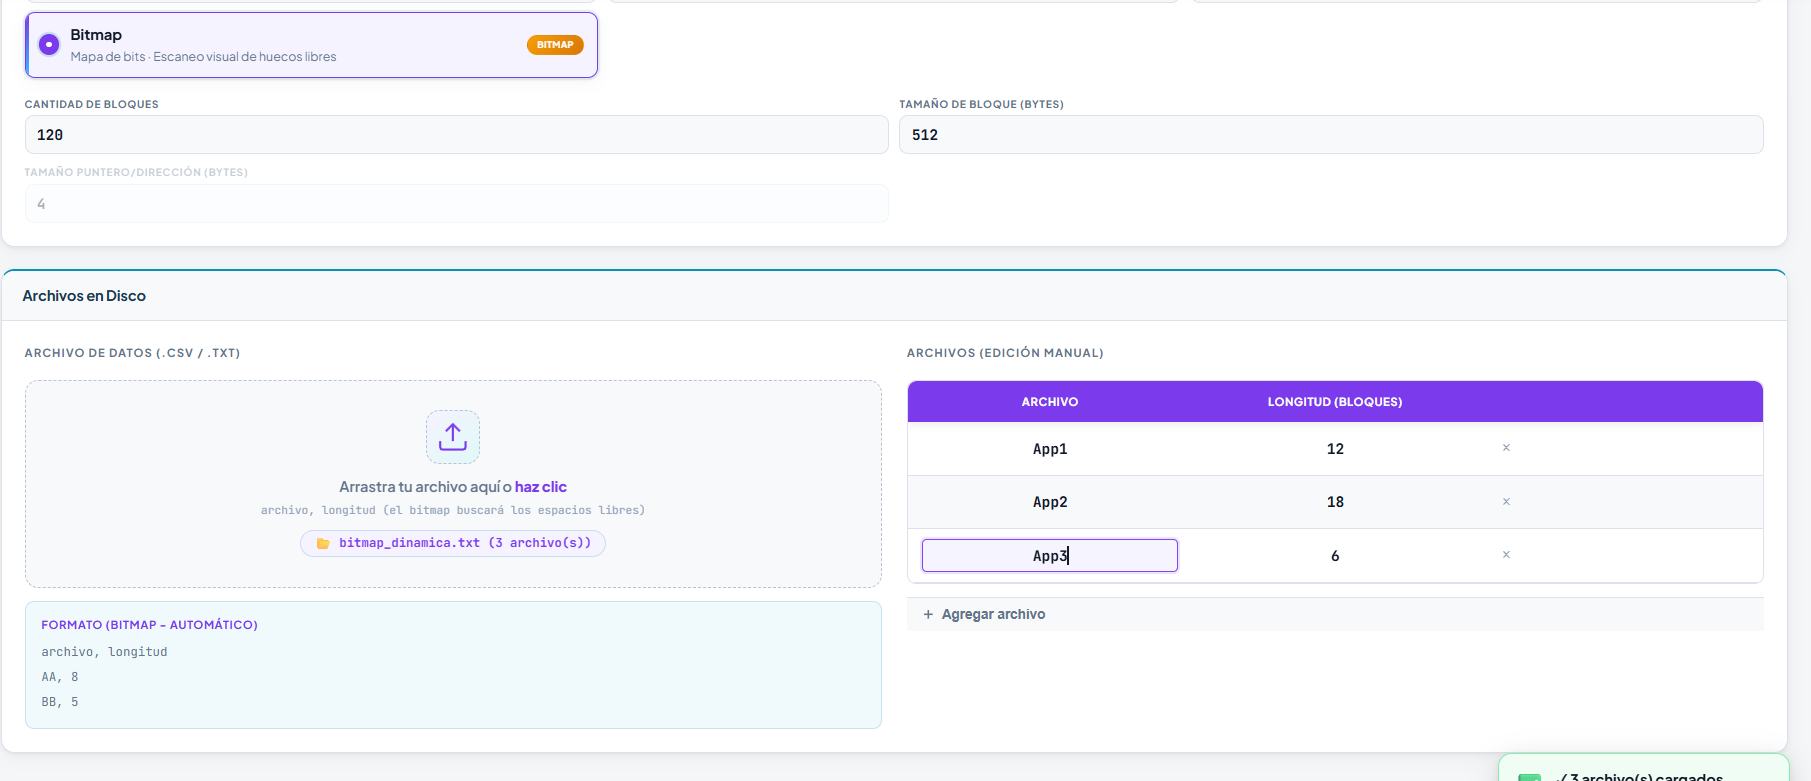
\includegraphics[width=0.9\textwidth]{imagenes/param_bitmap.png}
\end{figure}

\begin{figure}[H]
    \caption{\textit{El panel inferior del Mapa de Bits respondiendo en vivo a la asignación de archivos.}}
    \centering
    \vspace{0.3cm}
    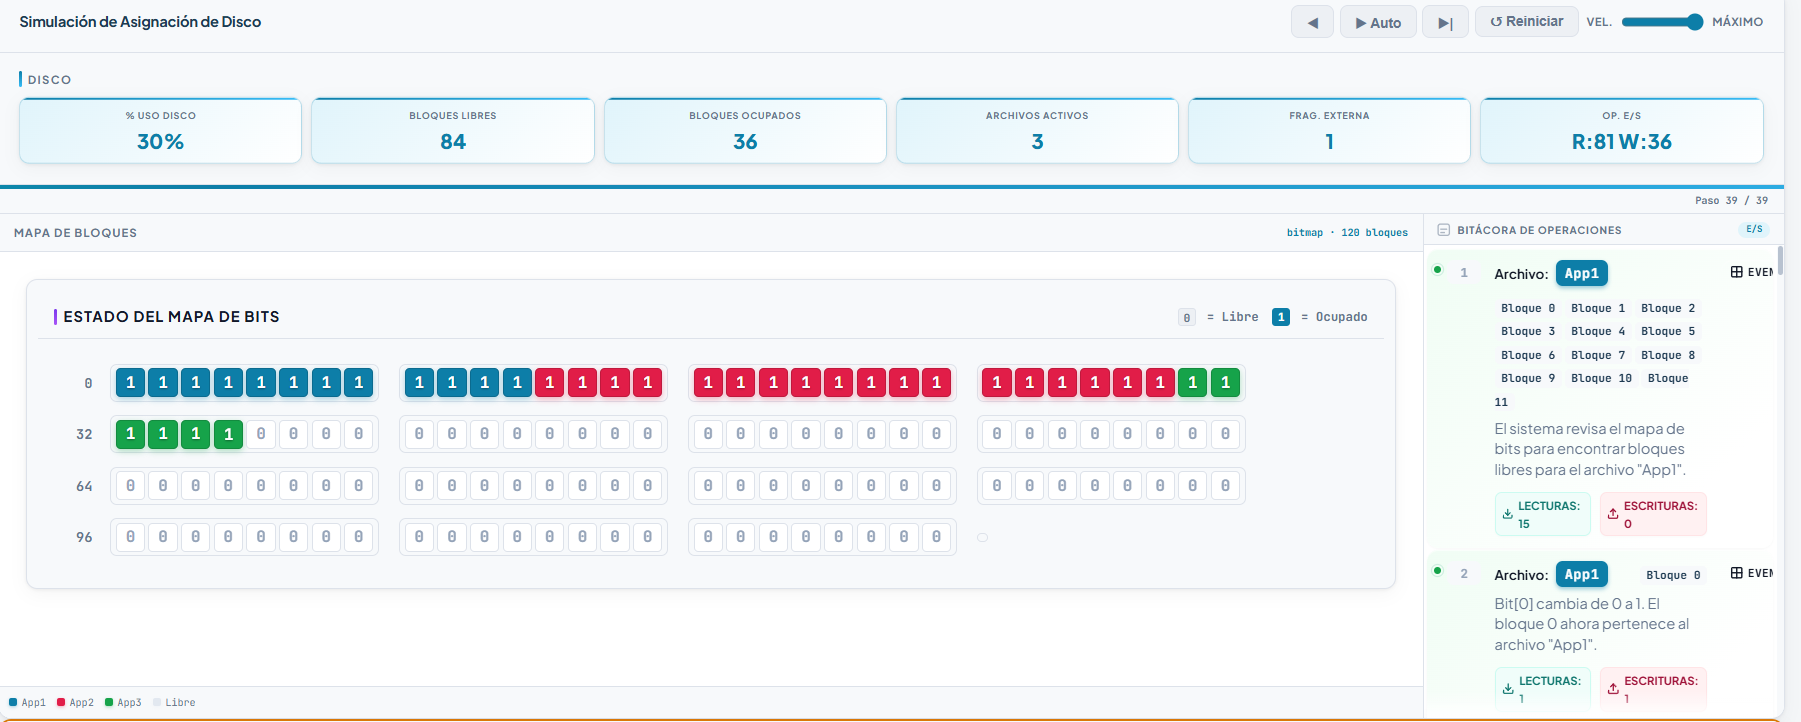
\includegraphics[width=1\textwidth]{imagenes/sim_bitmap.png}
\end{figure}

Durante la simulación, el panel inferior reflejó la transición binaria sincrónica. Los ceros lógicos cambiaron a unos simultáneamente a la ocupación gráfica de los bloques, demostrando la marcación inmediata del espacio en memoria.

\section{Conclusión}
El análisis visual corrobora que ninguna técnica resuelve de forma absoluta los desafíos del almacenamiento, requiriendo siempre un balance entre velocidad, mitigación de fragmentación y complejidad arquitectónica. En este contexto, el método FAT demuestra una alta eficiencia al maximizar la capacidad neta de los bloques físicos, eliminando la fragmentación externa al costo de centralizar su gestión y vulnerabilidad en una tabla única.

Por su parte, la indexación multi-nivel y las Extensiones abordan el manejo de grandes volúmenes de información desde enfoques distintos. La asignación indexada escala eficientemente estructurando jerarquías, aunque penaliza el rendimiento al exigir múltiples lecturas de peaje. En contraste, las Extensiones logran un equilibrio sobresaliente agrupando datos en porciones contiguas masivas, lo que optimiza la velocidad de lectura secuencial y justifica su adopción en arquitecturas contemporáneas.

Finalmente, la operación del mapa de bits expone cómo la asignación de espacio se procesa numéricamente a nivel de hardware, marcando la disponibilidad de forma binaria e inmediata. La convergencia de estos algoritmos en el simulador consolida los principios teóricos en métricas tangibles, demostrando que la elección de la estructura ideal depende estrictamente del tipo de carga de trabajo que el sistema operativo deba administrar.

\newpage
\section{Referencias}
\vspace{-0.5cm}
\setlength{\parindent}{0cm}

\noindent
\hangindent=1.27cm
Silberschatz, A., Galvin, P. B., \& Gagne, G. (2018). \textit{Operating system concepts} (10ma ed.). Wiley.

\vspace{0.3cm}
\noindent
\hangindent=1.27cm
Stallings, W. (2018). \textit{Operating Systems: Internals and Design Principles} (9na ed.). Pearson.

\vspace{1cm}
\setlength{\parindent}{1.27cm}
\section{Anexos}

\subsection{Anexo A: Repositorio del Proyecto}
\begin{center}
    \url{https://github.com/Abad-cyber/Sistema-del-nucleo-S.O..git}
\end{center}

\end{document}
